\section{Function\_\-Control\_\-Area Class Reference}
\label{classFunction__Control__Area}\index{Function_Control_Area@{Function\_\-Control\_\-Area}}
{\tt \#include $<$function\_\-control\_\-area.h$>$}

Inheritance diagram for Function\_\-Control\_\-Area:\begin{figure}[H]
\begin{center}
\leavevmode
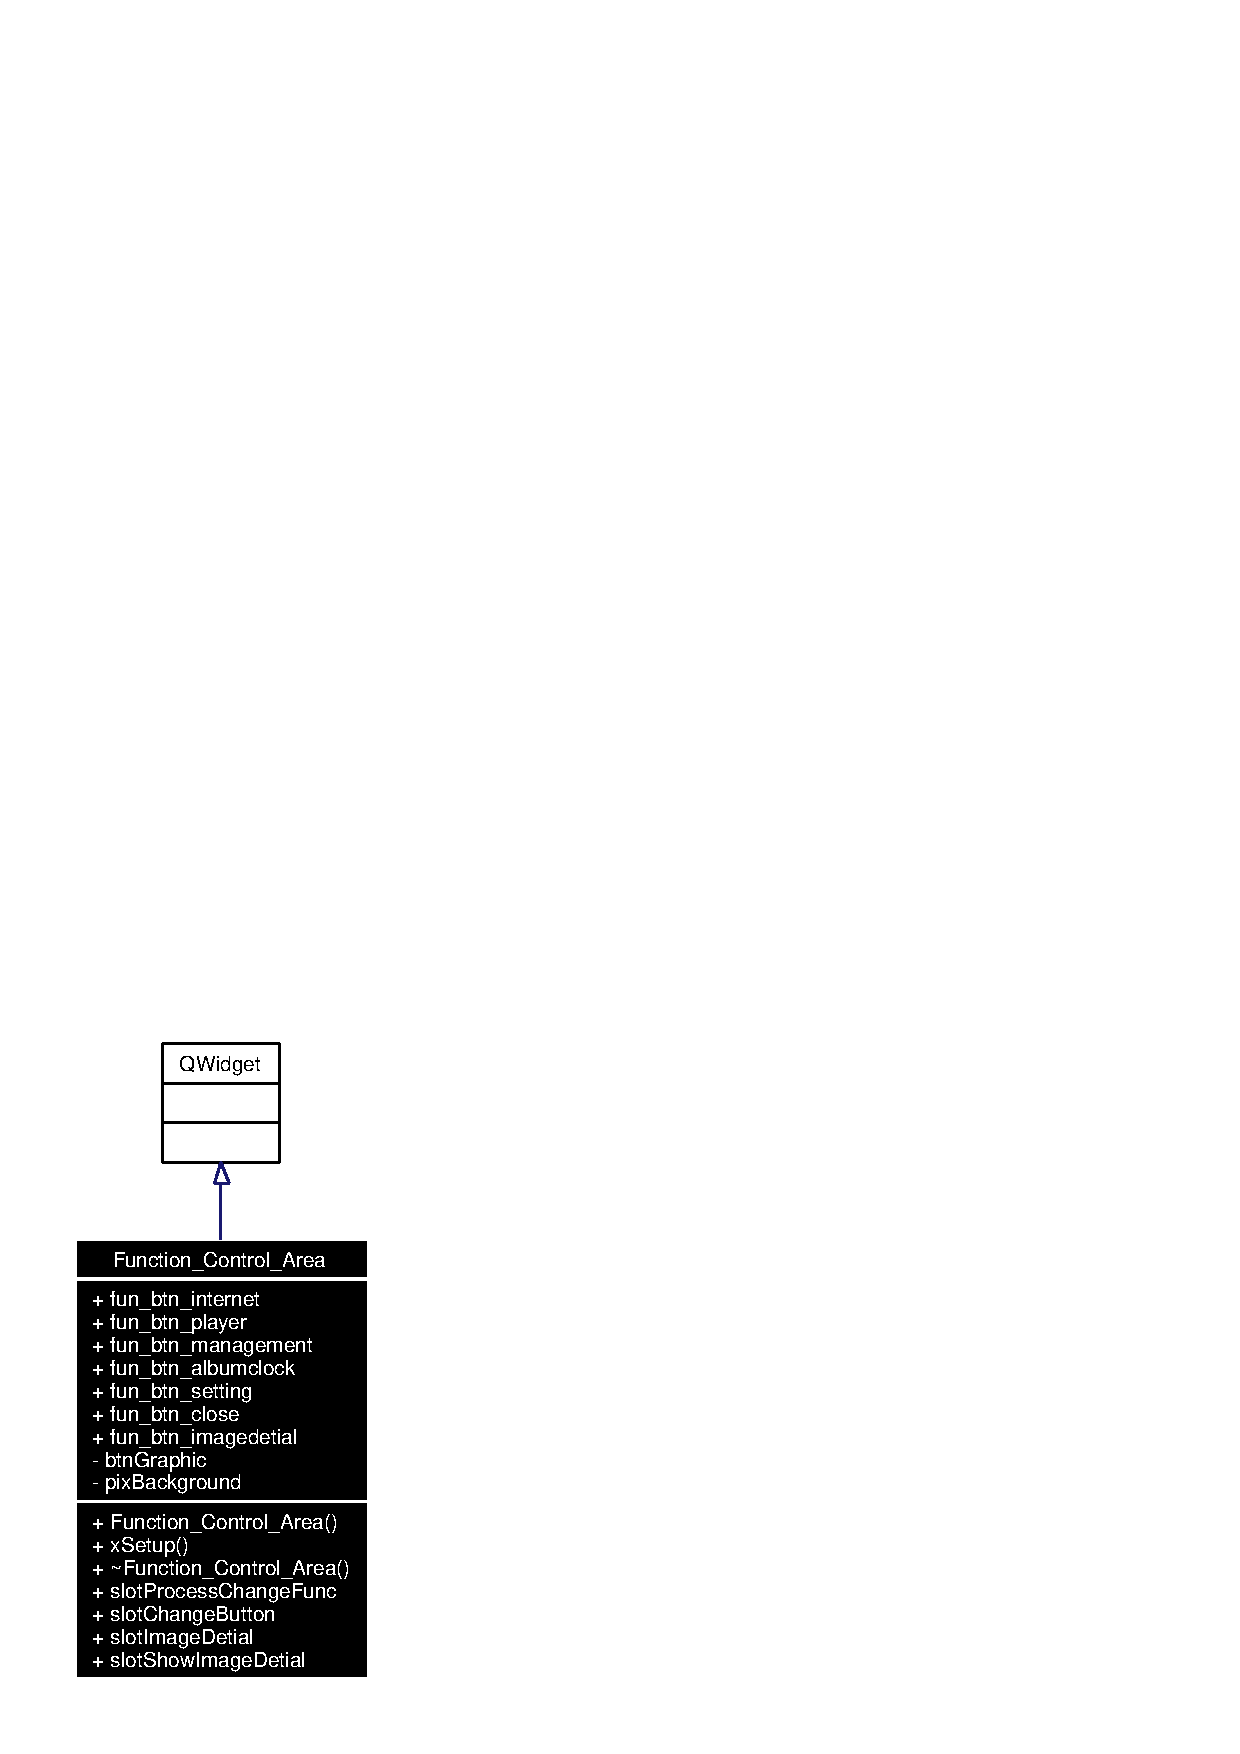
\includegraphics[width=88pt]{classFunction__Control__Area__inherit__graph}
\end{center}
\end{figure}
Collaboration diagram for Function\_\-Control\_\-Area:\begin{figure}[H]
\begin{center}
\leavevmode
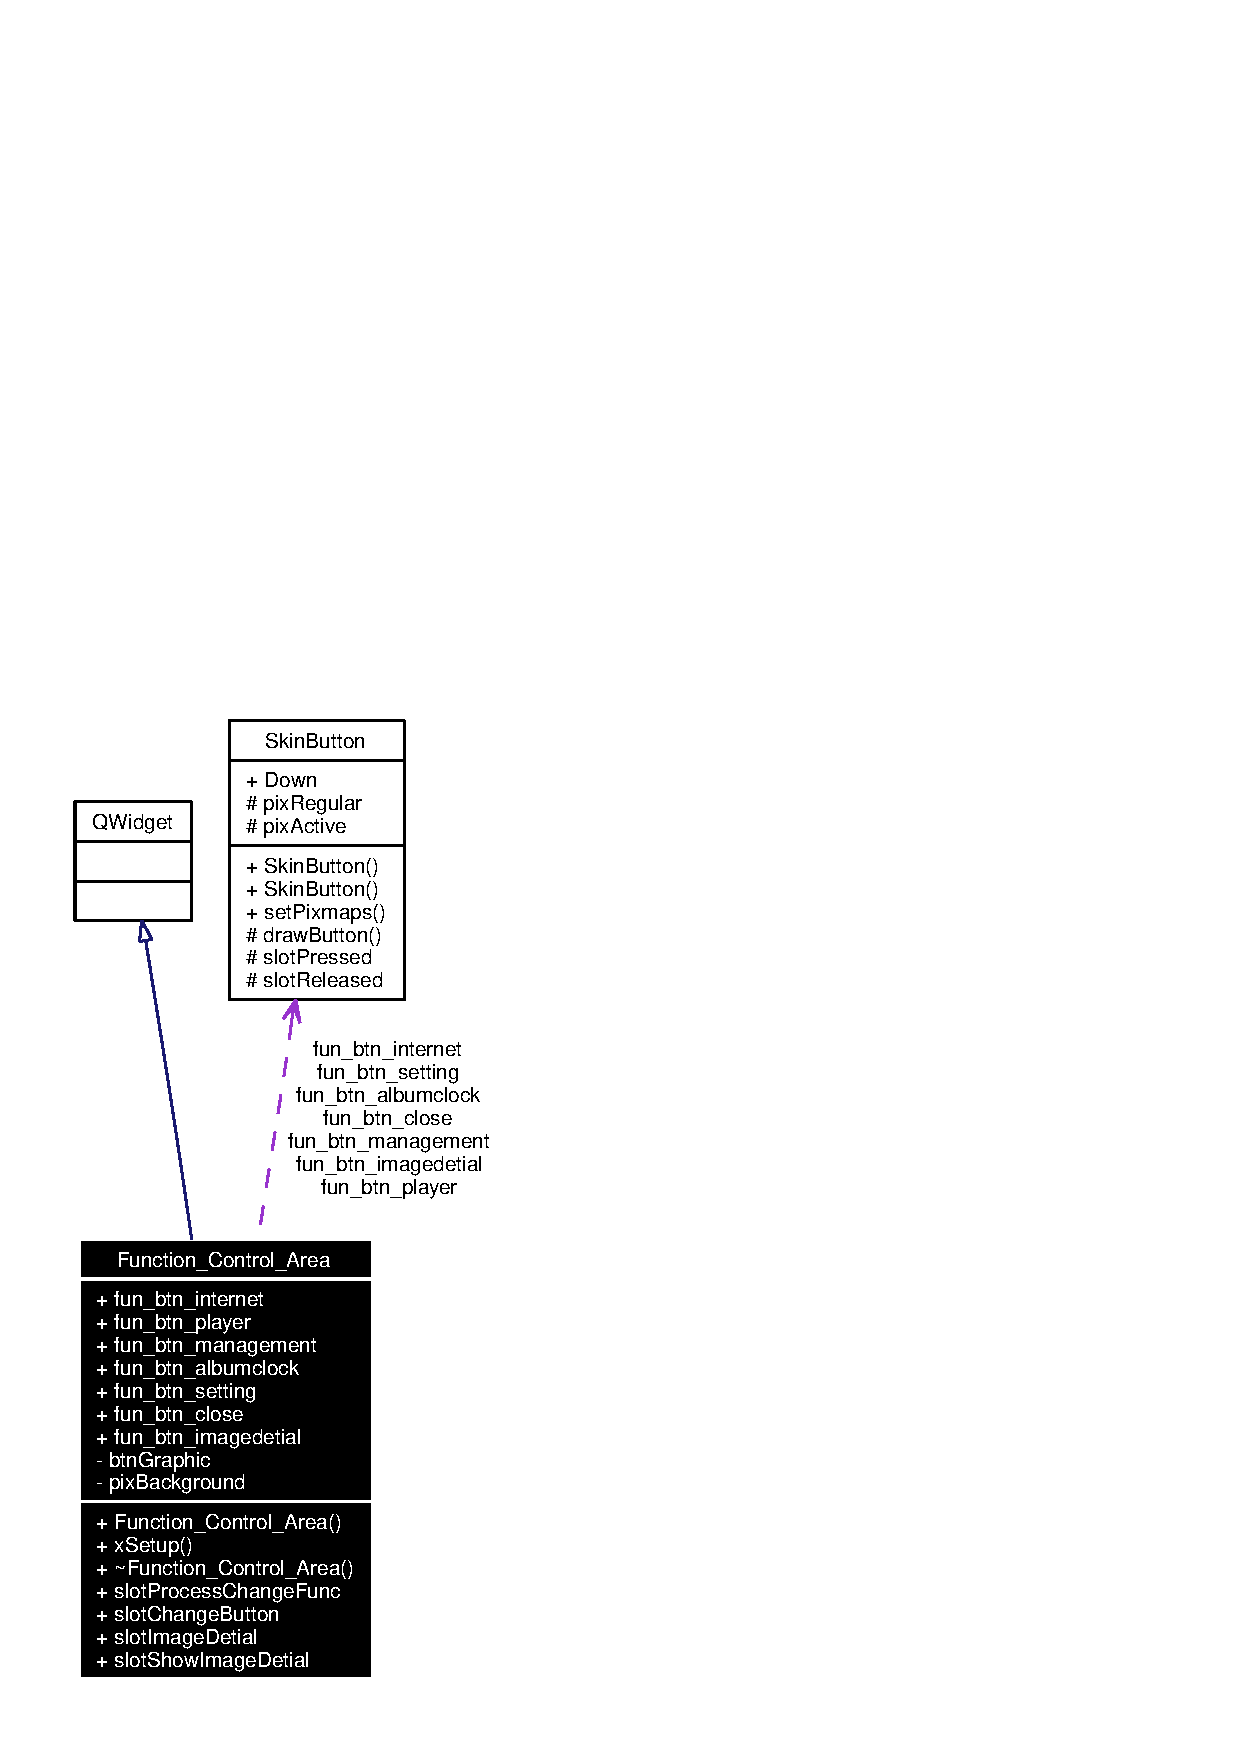
\includegraphics[width=125pt]{classFunction__Control__Area__coll__graph}
\end{center}
\end{figure}


\subsection{Detailed Description}
\begin{Desc}
\item[Author:]sonicat \end{Desc}




Definition at line 31 of file function\_\-control\_\-area.h.\subsection*{Public Slots}
\begin{CompactItemize}
\item 
void {\bf slot\-Process\-Change\-Func} ()
\item 
void {\bf slot\-Change\-Button} (int)
\item 
void {\bf slot\-Image\-Detial} ()
\item 
void {\bf slot\-Show\-Image\-Detial} ()
\end{CompactItemize}
\subsection*{Signals}
\begin{CompactItemize}
\item 
void {\bf signal\-Change\-Func} (int)
\item 
void {\bf signal\-Back\-To\-Management} ()
\end{CompactItemize}
\subsection*{Public Member Functions}
\begin{CompactItemize}
\item 
{\bf Function\_\-Control\_\-Area} ({\bf QWidget} $\ast$parent=0, const char $\ast$name=0)
\item 
void {\bf x\-Setup} ()
\item 
{\bf $\sim$Function\_\-Control\_\-Area} ()
\end{CompactItemize}
\subsection*{Public Attributes}
\begin{CompactItemize}
\item 
{\bf Skin\-Button} $\ast$ {\bf fun\_\-btn\_\-internet}
\item 
{\bf Skin\-Button} $\ast$ {\bf fun\_\-btn\_\-player}
\item 
{\bf Skin\-Button} $\ast$ {\bf fun\_\-btn\_\-management}
\item 
{\bf Skin\-Button} $\ast$ {\bf fun\_\-btn\_\-albumclock}
\item 
{\bf Skin\-Button} $\ast$ {\bf fun\_\-btn\_\-setting}
\item 
{\bf Skin\-Button} $\ast$ {\bf fun\_\-btn\_\-close}
\item 
{\bf Skin\-Button} $\ast$ {\bf fun\_\-btn\_\-imagedetial}
\end{CompactItemize}
\subsection*{Private Attributes}
\begin{CompactItemize}
\item 
QPixmap $\ast$ {\bf btn\-Graphic} [14]
\item 
QPixmap {\bf pix\-Background}
\end{CompactItemize}


\subsection{Constructor \& Destructor Documentation}
\index{Function_Control_Area@{Function\_\-Control\_\-Area}!Function_Control_Area@{Function\_\-Control\_\-Area}}
\index{Function_Control_Area@{Function\_\-Control\_\-Area}!Function_Control_Area@{Function\_\-Control\_\-Area}}
\subsubsection{\setlength{\rightskip}{0pt plus 5cm}Function\_\-Control\_\-Area::Function\_\-Control\_\-Area ({\bf QWidget} $\ast$ {\em parent} = 0, const char $\ast$ {\em name} = 0)}\label{classFunction__Control__Area_Function__Control__Areaa0}




Definition at line 22 of file function\_\-control\_\-area.cpp.

References x\-Setup().



\footnotesize\begin{verbatim}23  : QWidget(parent, name)
24 {
25         xSetup();
26 }
\end{verbatim}\normalsize 


Here is the call graph for this function:\begin{figure}[H]
\begin{center}
\leavevmode
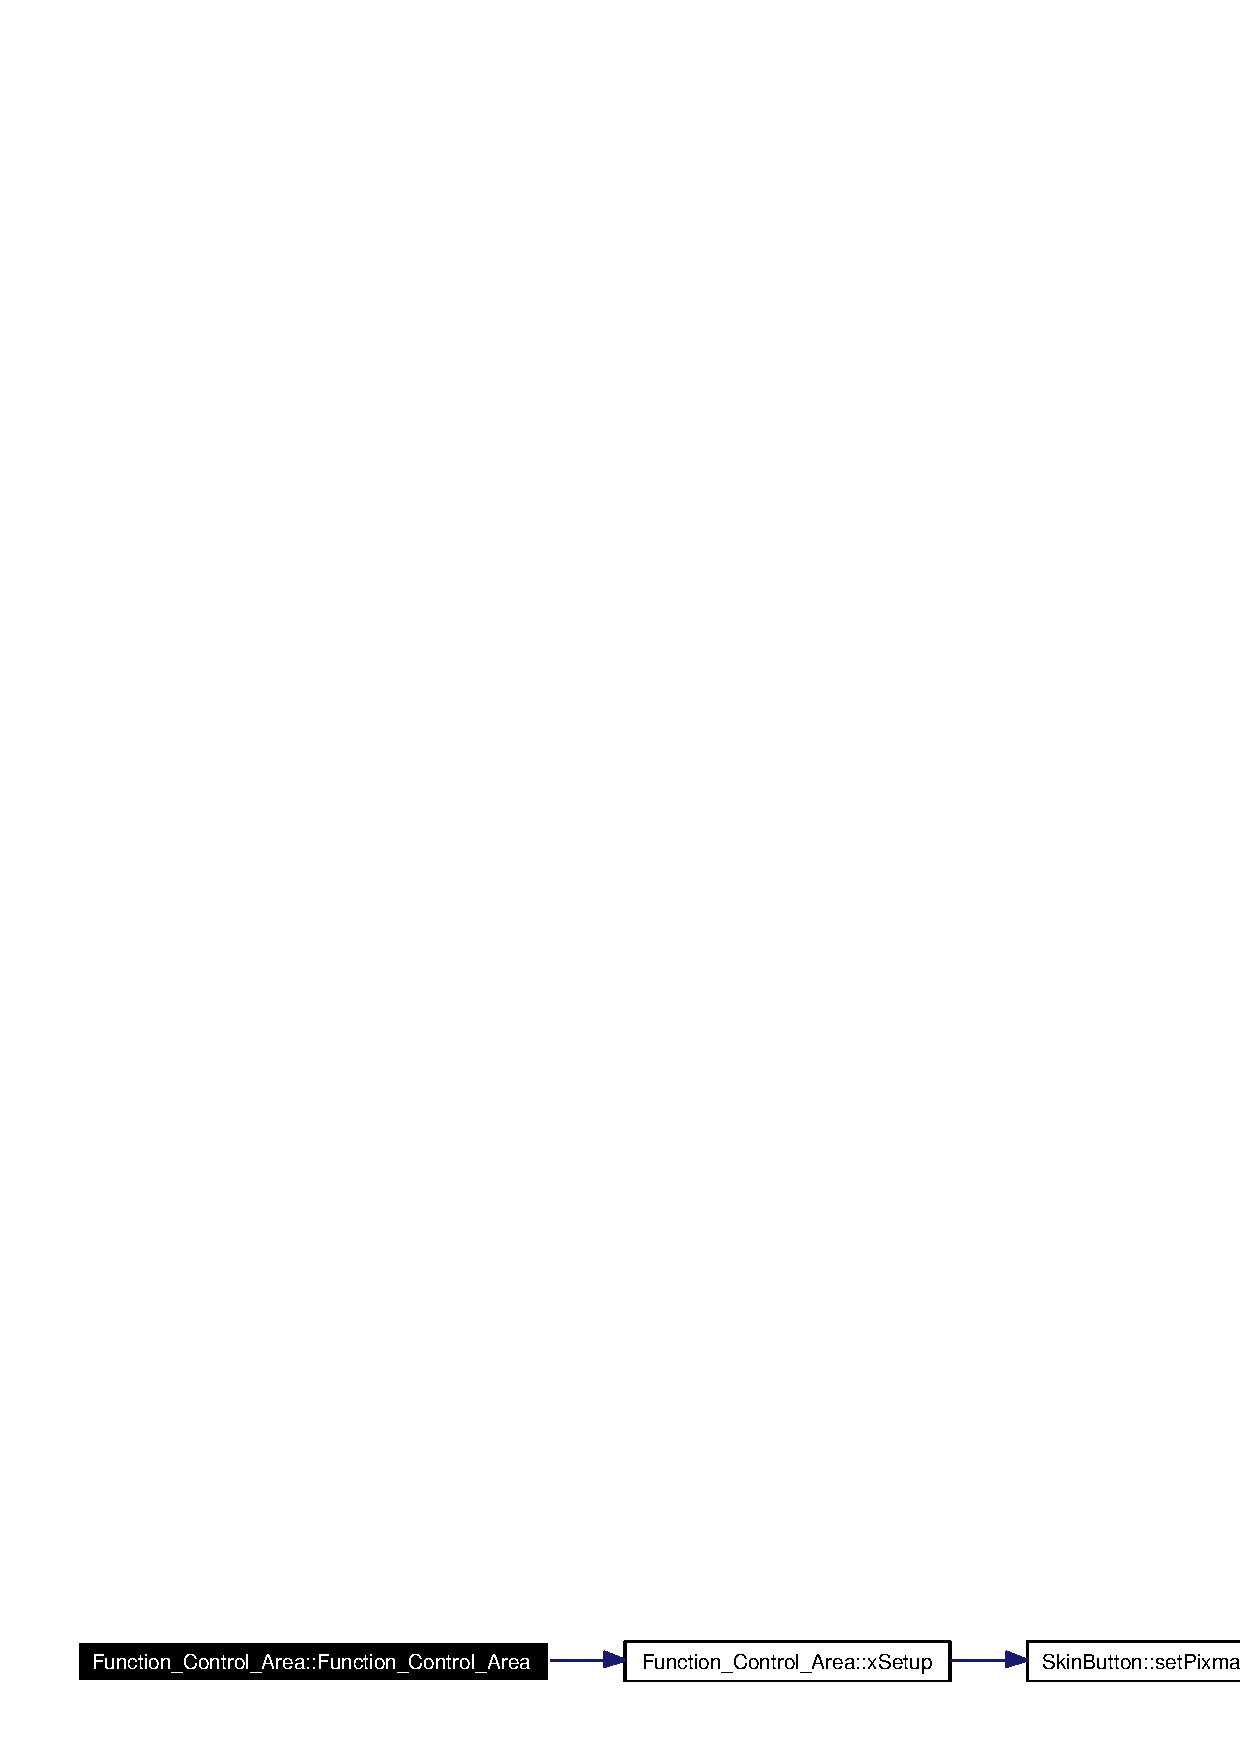
\includegraphics[width=308pt]{classFunction__Control__Area_Function__Control__Areaa0_cgraph}
\end{center}
\end{figure}
\index{Function_Control_Area@{Function\_\-Control\_\-Area}!~Function_Control_Area@{$\sim$Function\_\-Control\_\-Area}}
\index{~Function_Control_Area@{$\sim$Function\_\-Control\_\-Area}!Function_Control_Area@{Function\_\-Control\_\-Area}}
\subsubsection{\setlength{\rightskip}{0pt plus 5cm}Function\_\-Control\_\-Area::$\sim${\bf Function\_\-Control\_\-Area} ()}\label{classFunction__Control__Area_Function__Control__Areaa2}




Definition at line 29 of file function\_\-control\_\-area.cpp.



\footnotesize\begin{verbatim}30 {
31 }
\end{verbatim}\normalsize 


\subsection{Member Function Documentation}
\index{Function_Control_Area@{Function\_\-Control\_\-Area}!signalBackToManagement@{signalBackToManagement}}
\index{signalBackToManagement@{signalBackToManagement}!Function_Control_Area@{Function\_\-Control\_\-Area}}
\subsubsection{\setlength{\rightskip}{0pt plus 5cm}void Function\_\-Control\_\-Area::signal\-Back\-To\-Management ()\hspace{0.3cm}{\tt  [signal]}}\label{classFunction__Control__Area_Function__Control__Areal1}




Definition at line 104 of file function\_\-control\_\-area.moc.

Referenced by slot\-Image\-Detial().



\footnotesize\begin{verbatim}105 {
106     activate_signal( staticMetaObject()->signalOffset() + 1 );
107 }
\end{verbatim}\normalsize 
\index{Function_Control_Area@{Function\_\-Control\_\-Area}!signalChangeFunc@{signalChangeFunc}}
\index{signalChangeFunc@{signalChangeFunc}!Function_Control_Area@{Function\_\-Control\_\-Area}}
\subsubsection{\setlength{\rightskip}{0pt plus 5cm}void Function\_\-Control\_\-Area::signal\-Change\-Func (int)\hspace{0.3cm}{\tt  [signal]}}\label{classFunction__Control__Area_Function__Control__Areal0}




Definition at line 98 of file function\_\-control\_\-area.moc.

Referenced by slot\-Image\-Detial(), slot\-Process\-Change\-Func(), slot\-Show\-Image\-Detial(), and x\-Setup().



\footnotesize\begin{verbatim}99 {
100     activate_signal( staticMetaObject()->signalOffset() + 0, t0 );
101 }
\end{verbatim}\normalsize 
\index{Function_Control_Area@{Function\_\-Control\_\-Area}!slotChangeButton@{slotChangeButton}}
\index{slotChangeButton@{slotChangeButton}!Function_Control_Area@{Function\_\-Control\_\-Area}}
\subsubsection{\setlength{\rightskip}{0pt plus 5cm}void Function\_\-Control\_\-Area::slot\-Change\-Button (int)\hspace{0.3cm}{\tt  [slot]}}\label{classFunction__Control__Area_Function__Control__Areai1}




Definition at line 118 of file function\_\-control\_\-area.cpp.

References em\_\-albumclock, em\_\-close, em\_\-imagedetial, em\_\-internet, em\_\-management, em\_\-player, em\_\-setting, fun\_\-btn\_\-albumclock, fun\_\-btn\_\-close, fun\_\-btn\_\-imagedetial, fun\_\-btn\_\-internet, fun\_\-btn\_\-management, fun\_\-btn\_\-player, and fun\_\-btn\_\-setting.

Referenced by slot\-Image\-Detial(), slot\-Process\-Change\-Func(), slot\-Show\-Image\-Detial(), and x\-Setup().



\footnotesize\begin{verbatim}119 {
120    if(v==em_internet)
121    {
122      fun_btn_internet->show();
123      fun_btn_player->hide();
124      fun_btn_management->hide();
125      fun_btn_albumclock->hide();
126      fun_btn_setting->hide();
127      fun_btn_close->hide();
128      fun_btn_imagedetial->hide();
129    }
130    else if(v==em_player)
131    {
132      fun_btn_internet->hide();
133      fun_btn_player->show();
134      fun_btn_management->hide();
135      fun_btn_albumclock->hide();
136      fun_btn_setting->hide();
137      fun_btn_close->hide();
138      fun_btn_imagedetial->hide();
139    }
140    else if(v==em_management)
141    {
142      fun_btn_internet->hide();
143      fun_btn_player->hide();
144      fun_btn_management->show();
145      fun_btn_albumclock->hide();
146      fun_btn_setting->hide();
147      fun_btn_close->hide();
148      fun_btn_imagedetial->hide();
149    }
150    else if(v==em_albumclock)
151    {
152      fun_btn_internet->hide();
153      fun_btn_player->hide();
154      fun_btn_management->hide();
155      fun_btn_albumclock->show();
156      fun_btn_setting->hide();
157      fun_btn_close->hide();
158      fun_btn_imagedetial->hide();
159    }
160    else if(v==em_setting)
161    {
162      fun_btn_internet->hide();
163      fun_btn_player->hide();
164      fun_btn_management->hide();
165      fun_btn_albumclock->hide();
166      fun_btn_setting->show();
167      fun_btn_close->hide();
168      fun_btn_imagedetial->hide();
169    }
170    else if(v==em_close)
171    {
172      fun_btn_internet->hide();
173      fun_btn_player->hide();
174      fun_btn_management->hide();
175      fun_btn_albumclock->hide();
176      fun_btn_setting->hide();
177      fun_btn_close->show();
178      fun_btn_imagedetial->hide();
179    }
180    else if(v==em_imagedetial)
181    {
182     fun_btn_internet->hide();
183      fun_btn_player->hide();
184      fun_btn_management->hide();
185      fun_btn_albumclock->hide();
186      fun_btn_setting->hide();
187      fun_btn_close->hide();
188      fun_btn_imagedetial->show();
189    }
190 }
\end{verbatim}\normalsize 
\index{Function_Control_Area@{Function\_\-Control\_\-Area}!slotImageDetial@{slotImageDetial}}
\index{slotImageDetial@{slotImageDetial}!Function_Control_Area@{Function\_\-Control\_\-Area}}
\subsubsection{\setlength{\rightskip}{0pt plus 5cm}void Function\_\-Control\_\-Area::slot\-Image\-Detial ()\hspace{0.3cm}{\tt  [slot]}}\label{classFunction__Control__Area_Function__Control__Areai2}




Definition at line 192 of file function\_\-control\_\-area.cpp.

References em\_\-management, Global\-Setting, HDASSGlobal\-Setting::int\-HDASS\_\-FUNCTION\_\-STATE, signal\-Back\-To\-Management(), signal\-Change\-Func(), and slot\-Change\-Button().

Referenced by x\-Setup().



\footnotesize\begin{verbatim}193 {
194       //Back to em_management state
195       GlobalSetting.intHDASS_FUNCTION_STATE=em_management;
196       slotChangeButton(GlobalSetting.intHDASS_FUNCTION_STATE);
197       emit signalChangeFunc(GlobalSetting.intHDASS_FUNCTION_STATE);
198       emit signalBackToManagement();
199 }
\end{verbatim}\normalsize 
\index{Function_Control_Area@{Function\_\-Control\_\-Area}!slotProcessChangeFunc@{slotProcessChangeFunc}}
\index{slotProcessChangeFunc@{slotProcessChangeFunc}!Function_Control_Area@{Function\_\-Control\_\-Area}}
\subsubsection{\setlength{\rightskip}{0pt plus 5cm}void Function\_\-Control\_\-Area::slot\-Process\-Change\-Func ()\hspace{0.3cm}{\tt  [slot]}}\label{classFunction__Control__Area_Function__Control__Areai0}




Definition at line 108 of file function\_\-control\_\-area.cpp.

References Global\-Setting, HDASSGlobal\-Setting::int\-HDASS\_\-FUNCTION\_\-STATE, signal\-Change\-Func(), and slot\-Change\-Button().

Referenced by x\-Setup().



\footnotesize\begin{verbatim}109 {
110   //DAVID Process To Next Function
111   GlobalSetting.intHDASS_FUNCTION_STATE++;
112   GlobalSetting.intHDASS_FUNCTION_STATE%=6;
113   //qWarning("FunctionState::%d\n",GlobalSetting.intHDASS_FUNCTION_STATE);
114   slotChangeButton(GlobalSetting.intHDASS_FUNCTION_STATE);
115   emit signalChangeFunc(GlobalSetting.intHDASS_FUNCTION_STATE);
116 }
\end{verbatim}\normalsize 
\index{Function_Control_Area@{Function\_\-Control\_\-Area}!slotShowImageDetial@{slotShowImageDetial}}
\index{slotShowImageDetial@{slotShowImageDetial}!Function_Control_Area@{Function\_\-Control\_\-Area}}
\subsubsection{\setlength{\rightskip}{0pt plus 5cm}void Function\_\-Control\_\-Area::slot\-Show\-Image\-Detial ()\hspace{0.3cm}{\tt  [slot]}}\label{classFunction__Control__Area_Function__Control__Areai3}




Definition at line 201 of file function\_\-control\_\-area.cpp.

References em\_\-imagedetial, Global\-Setting, HDASSGlobal\-Setting::int\-HDASS\_\-FUNCTION\_\-STATE, signal\-Change\-Func(), and slot\-Change\-Button().



\footnotesize\begin{verbatim}202 {
203       GlobalSetting.intHDASS_FUNCTION_STATE=em_imagedetial;
204       slotChangeButton(GlobalSetting.intHDASS_FUNCTION_STATE);
205       emit signalChangeFunc(GlobalSetting.intHDASS_FUNCTION_STATE);
206 }
\end{verbatim}\normalsize 
\index{Function_Control_Area@{Function\_\-Control\_\-Area}!xSetup@{xSetup}}
\index{xSetup@{xSetup}!Function_Control_Area@{Function\_\-Control\_\-Area}}
\subsubsection{\setlength{\rightskip}{0pt plus 5cm}void Function\_\-Control\_\-Area::x\-Setup ()}\label{classFunction__Control__Area_Function__Control__Areaa1}




Definition at line 33 of file function\_\-control\_\-area.cpp.

References btn\-Graphic, fun\_\-btn\_\-albumclock, fun\_\-btn\_\-close, fun\_\-btn\_\-imagedetial, fun\_\-btn\_\-internet, fun\_\-btn\_\-management, fun\_\-btn\_\-player, fun\_\-btn\_\-setting, Global\-Setting, HDASSGlobal\-Setting::int\-HDASS\_\-FUNCTION\_\-STATE, pix\-Background, Skin\-Button::set\-Pixmaps(), signal\-Change\-Func(), slot\-Change\-Button(), slot\-Image\-Detial(), and slot\-Process\-Change\-Func().

Referenced by Function\_\-Control\_\-Area().



\footnotesize\begin{verbatim}34 {
35    QBitmap mask=QBitmap("/root/kde_application/hdass08/skin/function_control_masking.png");
36    setMask(mask);
37    //DAVID Setup Background;
38    pixBackground.load("/root/kde_application/hdass08/skin/FunctionAreaBackground.png");
39    setBackgroundPixmap(pixBackground);
40    //InitButton Graphic
41    btnGraphic[0]=new QPixmap("/root/kde_application/hdass08/skin/skin-function-button-internet.png");
42    btnGraphic[1]=new QPixmap("/root/kde_application/hdass08/skin/skin-function-button-internet-active.png");
43    btnGraphic[2]=new QPixmap("/root/kde_application/hdass08/skin/skin-function-button-player.png");
44    btnGraphic[3]=new QPixmap("/root/kde_application/hdass08/skin/skin-function-button-player-active.png");
45    btnGraphic[4]=new QPixmap("/root/kde_application/hdass08/skin/skin-function-button-management.png");
46    btnGraphic[5]=new QPixmap("/root/kde_application/hdass08/skin/skin-function-button-management-active.png");
47    btnGraphic[6]=new QPixmap("/root/kde_application/hdass08/skin/skin-function-button-albumclock.png");
48    btnGraphic[7]=new QPixmap("/root/kde_application/hdass08/skin/skin-function-button-albumclock-active.png");
49    btnGraphic[8]=new QPixmap("/root/kde_application/hdass08/skin/skin-function-button-setting.png");
50    btnGraphic[9]=new QPixmap("/root/kde_application/hdass08/skin/skin-function-button-setting-active.png");
51    btnGraphic[10]=new QPixmap("/root/kde_application/hdass08/skin/skin-function-button-close.png");
52    btnGraphic[11]=new QPixmap("/root/kde_application/hdass08/skin/skin-function-button-close-active.png");
53    btnGraphic[12]=new QPixmap("/root/kde_application/hdass08/skin/skin-function-button-imagedetial.png");
54    btnGraphic[13]=new QPixmap("/root/kde_application/hdass08/skin/skin-function-button-imagedetial-active.png");
55    
56    //Init Skinbutton
57    fun_btn_internet             =new SkinButton(this);
58    fun_btn_player              =new SkinButton(this);
59    fun_btn_management     =new SkinButton(this);
60    fun_btn_albumclock       =new SkinButton(this);
61    fun_btn_setting             =new SkinButton(this);
62    fun_btn_close               =new SkinButton(this);
63    fun_btn_imagedetial      =new SkinButton(this);
64    
65    fun_btn_internet->setPixmaps(btnGraphic[0],btnGraphic[1]);
66    fun_btn_internet->setGeometry(0,0,135,135);
67    fun_btn_internet->show();
68    
69    fun_btn_player->setPixmaps(btnGraphic[2],btnGraphic[3]);
70    fun_btn_player->setGeometry(0,0,135,135);
71    fun_btn_player->hide();
72    
73    fun_btn_management->setPixmaps(btnGraphic[4],btnGraphic[5]);
74    fun_btn_management->setGeometry(0,0,135,135);
75    fun_btn_management->hide();
76    
77    fun_btn_albumclock->setPixmaps(btnGraphic[6],btnGraphic[7]);
78    fun_btn_albumclock->setGeometry(0,0,135,135);
79    fun_btn_albumclock->hide();
80    
81    fun_btn_setting->setPixmaps(btnGraphic[8],btnGraphic[9]);
82    fun_btn_setting->setGeometry(0,0,135,135);
83    fun_btn_setting->hide();
84    
85    fun_btn_close->setPixmaps(btnGraphic[10],btnGraphic[11]);
86    fun_btn_close->setGeometry(0,0,135,135);
87    fun_btn_close->hide();
88    
89    fun_btn_imagedetial->setPixmaps(btnGraphic[12],btnGraphic[13]);
90    fun_btn_imagedetial->setGeometry(0,0,135,135);
91    fun_btn_imagedetial->hide();
92    
93    
94    
95    connect(fun_btn_internet,SIGNAL(released()),this,SLOT(slotProcessChangeFunc()));
96     connect(fun_btn_player,SIGNAL(released()),this,SLOT(slotProcessChangeFunc()));
97      connect(fun_btn_management,SIGNAL(released()),this,SLOT(slotProcessChangeFunc()));
98       connect(fun_btn_albumclock,SIGNAL(released()),this,SLOT(slotProcessChangeFunc()));
99        connect(fun_btn_setting,SIGNAL(released()),this,SLOT(slotProcessChangeFunc()));
100         connect(fun_btn_close,SIGNAL(released()),this,SLOT(slotProcessChangeFunc()));
101         connect(fun_btn_imagedetial,SIGNAL(released()),this,SLOT(slotImageDetial()));
102       //DAVID Set the Function Control Area State
103       
104       slotChangeButton(GlobalSetting.intHDASS_FUNCTION_STATE);
105       emit signalChangeFunc(GlobalSetting.intHDASS_FUNCTION_STATE);
106 }
\end{verbatim}\normalsize 


Here is the call graph for this function:\begin{figure}[H]
\begin{center}
\leavevmode
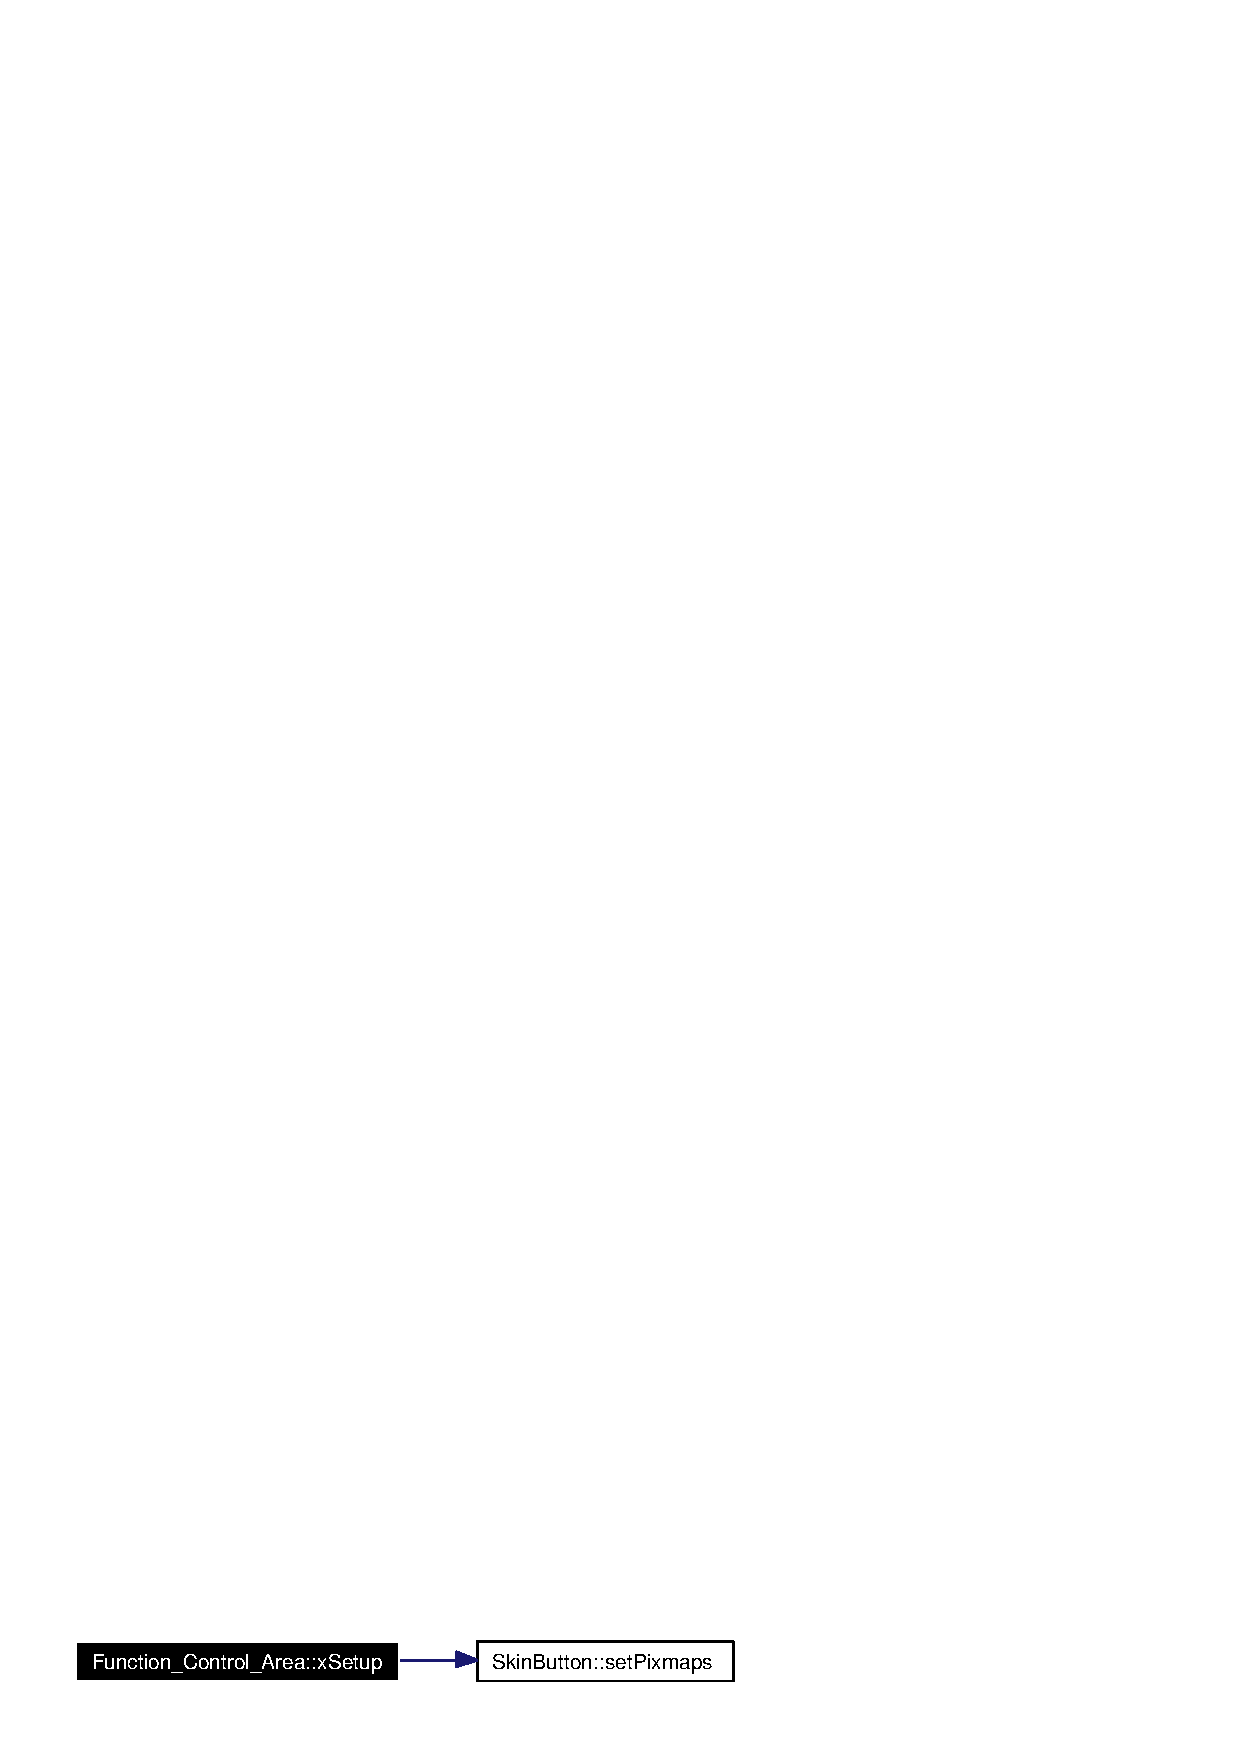
\includegraphics[width=176pt]{classFunction__Control__Area_Function__Control__Areaa1_cgraph}
\end{center}
\end{figure}


\subsection{Member Data Documentation}
\index{Function_Control_Area@{Function\_\-Control\_\-Area}!btnGraphic@{btnGraphic}}
\index{btnGraphic@{btnGraphic}!Function_Control_Area@{Function\_\-Control\_\-Area}}
\subsubsection{\setlength{\rightskip}{0pt plus 5cm}QPixmap$\ast$ {\bf Function\_\-Control\_\-Area::btn\-Graphic}[14]\hspace{0.3cm}{\tt  [private]}}\label{classFunction__Control__Area_Function__Control__Arear0}




Definition at line 49 of file function\_\-control\_\-area.h.

Referenced by x\-Setup().\index{Function_Control_Area@{Function\_\-Control\_\-Area}!fun_btn_albumclock@{fun\_\-btn\_\-albumclock}}
\index{fun_btn_albumclock@{fun\_\-btn\_\-albumclock}!Function_Control_Area@{Function\_\-Control\_\-Area}}
\subsubsection{\setlength{\rightskip}{0pt plus 5cm}{\bf Skin\-Button} $\ast$ {\bf Function\_\-Control\_\-Area::fun\_\-btn\_\-albumclock}}\label{classFunction__Control__Area_Function__Control__Areao3}




Definition at line 39 of file function\_\-control\_\-area.h.

Referenced by slot\-Change\-Button(), and x\-Setup().\index{Function_Control_Area@{Function\_\-Control\_\-Area}!fun_btn_close@{fun\_\-btn\_\-close}}
\index{fun_btn_close@{fun\_\-btn\_\-close}!Function_Control_Area@{Function\_\-Control\_\-Area}}
\subsubsection{\setlength{\rightskip}{0pt plus 5cm}{\bf Skin\-Button} $\ast$ {\bf Function\_\-Control\_\-Area::fun\_\-btn\_\-close}}\label{classFunction__Control__Area_Function__Control__Areao5}




Definition at line 39 of file function\_\-control\_\-area.h.

Referenced by slot\-Change\-Button(), and x\-Setup().\index{Function_Control_Area@{Function\_\-Control\_\-Area}!fun_btn_imagedetial@{fun\_\-btn\_\-imagedetial}}
\index{fun_btn_imagedetial@{fun\_\-btn\_\-imagedetial}!Function_Control_Area@{Function\_\-Control\_\-Area}}
\subsubsection{\setlength{\rightskip}{0pt plus 5cm}{\bf Skin\-Button} $\ast$ {\bf Function\_\-Control\_\-Area::fun\_\-btn\_\-imagedetial}}\label{classFunction__Control__Area_Function__Control__Areao6}




Definition at line 39 of file function\_\-control\_\-area.h.

Referenced by slot\-Change\-Button(), and x\-Setup().\index{Function_Control_Area@{Function\_\-Control\_\-Area}!fun_btn_internet@{fun\_\-btn\_\-internet}}
\index{fun_btn_internet@{fun\_\-btn\_\-internet}!Function_Control_Area@{Function\_\-Control\_\-Area}}
\subsubsection{\setlength{\rightskip}{0pt plus 5cm}{\bf Skin\-Button}$\ast$ {\bf Function\_\-Control\_\-Area::fun\_\-btn\_\-internet}}\label{classFunction__Control__Area_Function__Control__Areao0}




Definition at line 39 of file function\_\-control\_\-area.h.

Referenced by slot\-Change\-Button(), and x\-Setup().\index{Function_Control_Area@{Function\_\-Control\_\-Area}!fun_btn_management@{fun\_\-btn\_\-management}}
\index{fun_btn_management@{fun\_\-btn\_\-management}!Function_Control_Area@{Function\_\-Control\_\-Area}}
\subsubsection{\setlength{\rightskip}{0pt plus 5cm}{\bf Skin\-Button} $\ast$ {\bf Function\_\-Control\_\-Area::fun\_\-btn\_\-management}}\label{classFunction__Control__Area_Function__Control__Areao2}




Definition at line 39 of file function\_\-control\_\-area.h.

Referenced by slot\-Change\-Button(), and x\-Setup().\index{Function_Control_Area@{Function\_\-Control\_\-Area}!fun_btn_player@{fun\_\-btn\_\-player}}
\index{fun_btn_player@{fun\_\-btn\_\-player}!Function_Control_Area@{Function\_\-Control\_\-Area}}
\subsubsection{\setlength{\rightskip}{0pt plus 5cm}{\bf Skin\-Button} $\ast$ {\bf Function\_\-Control\_\-Area::fun\_\-btn\_\-player}}\label{classFunction__Control__Area_Function__Control__Areao1}




Definition at line 39 of file function\_\-control\_\-area.h.

Referenced by slot\-Change\-Button(), and x\-Setup().\index{Function_Control_Area@{Function\_\-Control\_\-Area}!fun_btn_setting@{fun\_\-btn\_\-setting}}
\index{fun_btn_setting@{fun\_\-btn\_\-setting}!Function_Control_Area@{Function\_\-Control\_\-Area}}
\subsubsection{\setlength{\rightskip}{0pt plus 5cm}{\bf Skin\-Button} $\ast$ {\bf Function\_\-Control\_\-Area::fun\_\-btn\_\-setting}}\label{classFunction__Control__Area_Function__Control__Areao4}




Definition at line 39 of file function\_\-control\_\-area.h.

Referenced by slot\-Change\-Button(), and x\-Setup().\index{Function_Control_Area@{Function\_\-Control\_\-Area}!pixBackground@{pixBackground}}
\index{pixBackground@{pixBackground}!Function_Control_Area@{Function\_\-Control\_\-Area}}
\subsubsection{\setlength{\rightskip}{0pt plus 5cm}QPixmap {\bf Function\_\-Control\_\-Area::pix\-Background}\hspace{0.3cm}{\tt  [private]}}\label{classFunction__Control__Area_Function__Control__Arear1}




Definition at line 50 of file function\_\-control\_\-area.h.

Referenced by x\-Setup().

The documentation for this class was generated from the following files:\begin{CompactItemize}
\item 
{\bf function\_\-control\_\-area.h}\item 
{\bf function\_\-control\_\-area.moc}\item 
{\bf function\_\-control\_\-area.cpp}\end{CompactItemize}
